%%%%%%%%%%%%%%教案头%%%%%%%%%%%%%%%%%%%%%%%%%%%%%%%
\mode<article>{

\begin{longtable}{|m{20mm}|m{20mm}|m{20mm}|m{20mm}|m{20mm}|m{28mm}|}
\caption*{\huge 教案头}\\
\hline
\endfirsthead
\multicolumn{6}{l}{(续表)}\\
\hline
\endhead
\hline
\multicolumn{6}{l}{\itshape 接下一页表格.......}\\ [2ex]
\endfoot
\hline
\endlastfoot
\centering{授课单元}&\multicolumn{3}{m{60mm}|}{\centering 2.6控制系统的时域分析2.6.1脉新华路响应和阶路响应2.6.2时域性能指标2.6.3一阶系统的动态响应}&\centering{授课日期}&2014年03月13日 \\
\hline
\centering 授课地点 & \multicolumn{3}{m{60mm}|}{B6-204}&\centering 授课学时 & 2 \\
\hline
& \multicolumn{2}{m{40mm}|}{能力目标} & \multicolumn{2}{m{40mm}|}{知识目标}&素质目标 \\
\cline{2-6}
\centering 教学目标&\multicolumn{2}{m{40mm}|}{\begin{enumerate}
\item 能够分析一阶系统的动态响应
\end{enumerate} }&\multicolumn{2}{m{40mm}|}{\begin{enumerate}
\item 了解脉冲响应函数和阶跃响应函数
\item 了解时域性能指标
\end{enumerate}} & {\qquad}\\
\hline
\centering 能力训练任务或案例 &\multicolumn{5}{m{108mm}|}{ }\\
\hline
\centering 教学重点 & \multicolumn{5}{m{108mm}|}{\begin{enumerate}
\item 一阶系统的动态响应
\end{enumerate}}\\
\hline
\centering 教学难点与解决办法 &\multicolumn{5}{m{108mm}|}{\begin{enumerate}
\item 难点:一阶系统的动态响应分析
\item 解决方法:用实例进行分析讲解
\end{enumerate}}\\
\hline
\centering 德育内容 &\multicolumn{5}{m{108mm}|}{无}\\
\hline
 &教材 & \multicolumn{4}{m{88mm}|}{计算机控制原理与应用}\\
\cline{2-6}& 教学资源 &\multicolumn{4}{m{88mm}|}{PPT}\\
\cline{2-6}\centering 使用的教学材料& 主要教学仪器设备和工具等 &\multicolumn{4}{m{88mm}|}{投影机、MATLAB}\\
\cline{2-6}& 主要耗材 &\multicolumn{4}{m{88mm}|}{无}\\
\hline
\centering 教学模式 &\multicolumn{2}{m{40mm}|}{知识讲授}&\centering 教学手段 &\multicolumn{2}{m{48mm}|}{多媒体教学}\\
\hline
\centering 学生成果与过程考核方式 &\multicolumn{5}{m{108mm}|}{无}
\end{longtable}
\clearpage

%%%%%%%%%%%%%%%教学实施过程%%%%%%%%%%%%%%%%%%%%%%%%%%%%
\begin{landscape}

\begin{longtable}{|m{10mm}|m{50mm}|m{50mm}|m{50mm}|m{15mm}|}
\caption*{\huge 教学组织与实施}\\
\hline
\endfirsthead
\multicolumn{5}{l}{\small 接上页}\\
\hline
\multicolumn{1}{|c|}{步骤}&\multicolumn{1}{c|}{教学内容}&\multicolumn{1}{c|}{教师活动}&\multicolumn{1}{c|}{学生活动}&\multicolumn{1}{c|}{时间}\\
\hline
\endhead

\multicolumn{5}{r}{\small 接下页}\\
\endfoot
\hline
\endlastfoot
\multicolumn{1}{|c|}{步骤}&\multicolumn{1}{c|}{教学内容}&\multicolumn{1}{c|}{教师活动}&\multicolumn{1}{c|}{学生活动}&\multicolumn{1}{c|}{时间}\\\hline
讲解&\begin{enumerate}
\item 脉冲响应和阶跃响应
\end{enumerate} &\begin{enumerate}
\item 讲解分析单位脉冲响应和阶跃响应函数
\end{enumerate} &\begin{enumerate}
\item 学生倾听并记录
\end{enumerate} &20 \\\hline
讲解&\begin{enumerate}
\item 时域性能指标
\end{enumerate}
 &\begin{enumerate}
\item 通过图示讲解时域性能指标
\end{enumerate} &\begin{enumerate}
\item 学生倾听并记录
\end{enumerate} &25 \\\hline
讲解&\begin{enumerate}
\item 一阶系统的数学模型
\end{enumerate}
&\begin{enumerate}
\item 讲解一阶系统的数学模型
\end{enumerate} &\begin{enumerate}
\item 学生倾听并记录
\end{enumerate} &10 \\\hline
讲解&\begin{enumerate}
\item 一阶系统的单位阶跃响应
\end{enumerate}
 &\begin{enumerate}
\item 讲解阶系统的单位阶跃响应分析
\end{enumerate} &\begin{enumerate}
\item 学生记录笔记
\end{enumerate} &20 \\\hline
讲解&
\begin{enumerate}
\item 一阶系统的单位脉冲响应
\end{enumerate}
 &\begin{enumerate}
\item 讲解一阶系统的单位脉冲响应分析
\end{enumerate} &\begin{enumerate}
\item 学生记录笔记
\end{enumerate} &10 \\\hline
\centering 本次课总结(评价)&总结本课程内容 &进行知识总结 &学生倾听 &5 \\\hline
\centering 学生学习笔记或工单等检查情况&\multicolumn{4}{m{165mm}|}{\quad}\\\hline
\centering 课后作业&\multicolumn{4}{m{165mm}|}{2-19,2-20,2-21}\\\hline
\centering 教学体会&\multicolumn{4}{m{165mm}|}{\quad}\\
\end{longtable}

\end{landscape}
\clearpage
%%%%%%%%%%%%%%%%%%%%板书设计%%%%%%%%%%%%%%%%%%%%%%%%%%
\lecture{传递函数与信号流图}{chuandihanshu}
\begin{center}
{\huge 板书设计}
\end{center}
}
\mode<presentation>{ \section{控制系统的时域分析}
 \subsection{一阶系统的动态响应}}
 \begin{frame}{脉冲响应}
 \begin{block}{}
 \begin{itemize}
 \item<+-> 线性定常系统的传递函数为:$G(s)$
 \[r(t)=L^{-1}[R(s)]\]
 \item<+-> 则系统输出为:
 \[C(s)=G(s)R(s)\]
 \end{itemize}
 \end{block}
 \end{frame}
 
 \begin{frame}
 \begin{block}{}
 \begin{itemize}
 \item<+-> 输入为单位脉冲函数$\delta(t)$,输出记为$g(t)$,则:
 \[L[\delta]=1\]
 \[C(s)=G(s)\cdot 1\]
 \item<+-> 得:
 \[c(t)=g(t)\]
\end{itemize}  
\end{block}
\end{frame}

\begin{frame}
\begin{block}{}
\begin{itemize}
\item<+-> 系统传递函数等于单位脉冲函数$g(t)$的拉氏变换,即:
\[G(s)=L[g(t)]\]
\item<+-> 单位脉冲函数$g(t)$是传递函数$G(s)$拉氏逆变换,即:
\[g(t)=L^{-1}[G(s)]\]
\end{itemize}
\end{block}
\end{frame}
\begin{frame}
\begin{block}{}
推广:
\begin{eqnarray*}
c(t)&=&L^{-1}[C(s)]\\
&=&L^{-1}[G(s)R(s)]\\
&=&\int^{\infty}_{0}g(t-\tau)r(\tau)d\tau \\
&=&\int^{\infty}_{0}r(t-\tau)g(\tau)d\tau
\end{eqnarray*}
\end{block}
\end{frame}
\begin{frame}{阶跃响应}
\begin{block}{}
\begin{eqnarray*}
L[u(t)]=\frac{1}{s}\\
C(s)=G(s)R(s)=G(s)\frac{1}{s}=H(s)\\
h(t)=L^{-1}[C(s)]=L^{-1}[H(s)]=L^{-1}[\frac{G(s)}{s}]\\
h(t)=L^{-1}[\frac{G(s)}{s}]=\int^t_0g(t)dt
\end{eqnarray*}
\end{block}
\end{frame}
\begin{frame}
\begin{block}{}
\begin{eqnarray*}
G(s)=sH(s)\\
g(t)=L^{-1}[G(s)]=L^{-1}[sH(s)]=\frac{dh(t)}{dt}
\end{eqnarray*}
\end{block}
\end{frame}
\begin{frame}{时域性能指标}
\begin{block}{具有误差振荡的单位阶跃响应}
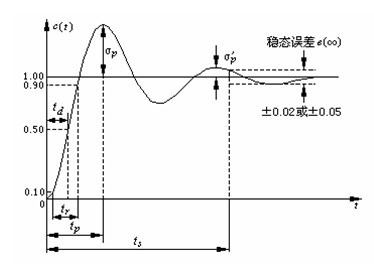
\includegraphics[scale=0.8]{danweijiyao}
\end{block}
\end{frame}
\begin{frame}
\begin{block}{}
\begin{itemize}
\item<+-> 延迟时间$t_d$:达到终值一半所需要的时间
\item<+-> 上升时间$t_r$:从终值的10\%到90\%所需要的时间
\item<+-> 峰值时间$t_p$:终值达到超调量的第一个峰值的时间
\item<+-> 最大超调量$M_p$:
\[M_p\%=\frac{c(t_p)-c(\infty)}{c(\infty)}\%\]
\end{itemize}
\end{block}
\end{frame}
\begin{frame}
\begin{block}{具有单调变化的单位阶跃响应}
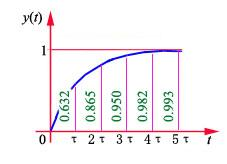
\includegraphics[scale=1.2]{onejieyaoimpulse}
\end{block}
\end{frame}
\begin{frame}{一阶系统的动态响应}
\begin{block}{一阶系统的数学模型}
\[\Phi(s)=\frac{V_2(s)}{V_1(s)}=\frac{1}{RCs+1}=\frac{1}{Ts+1}\]
其中:$T=RC$
\end{block}
\end{frame}
\begin{frame}{一阶系统的动态响应}
\begin{block}{一阶系统的单位阶跃响应}
\begin{eqnarray*}
r(t)=u(t)\\
R(s)=\frac{1}{s}\\
C(s)=\Phi(s)R(s)=\frac{1}{Ts+1}\cdot\frac{1}{s}\\
C(s)=\frac{1}{s(Ts+1)}=\frac{1}{s}-\frac{T}{Ts+1}\\
c(t)=L^{-1}[C(s)]=1-e^{-\frac{t}{T}},t\geq 0
\end{eqnarray*}
\end{block}
\end{frame}
\begin{frame}
\begin{block}{系统特性}
\begin{itemize}
\item<+-> $T$为时间常数,反映系统的惯性
\item<+-> $T$越小,系统惯性越小,系统响应越快
\item<+-> $t_s=0.3T$
\item<+-> $t_d=0.69T$
\item<+-> $t_r=2.20T$
\end{itemize}
\end{block}
\end{frame}
\begin{frame}{一阶系统的单位斜坡响应}
\begin{block}{}
\begin{eqnarray*}
C(s)=\Phi(s)R(s)=\frac{1}{Ts+1}\cdot\frac{1}{s^2}\\
C(s)=\frac{1}{s^2(Ts+1)}=\frac{1}{s^2}-\frac{T}{s}+
\frac{T^2}{Ts+1}\\
c(t)=L^{-1}[C(s)]=(t-T)+Te^{-\frac{t}{T}},t\geq 0
\end{eqnarray*}
\end{block}
\end{frame}
\begin{frame}{一阶系统的单脉冲响应}
\begin{block}{}
\begin{eqnarray*}
C(s)=\Phi(s)R(s)=\frac{1}{Ts+1}\\
c(t)=L^{-1}[C(s)]=\frac{1}{T}e^{-\frac{t}{T}},t\geq 0
\end{eqnarray*}
\end{block}
\end{frame}